\documentclass[conference]{IEEEtran}
\IEEEoverridecommandlockouts
% The preceding line is only needed to identify funding in the first footnote. If that is unneeded, please comment it out.
\usepackage{cite}
\usepackage{amsmath,amssymb,amsfonts}
\usepackage{algorithmic}
\usepackage{graphicx}
\usepackage{textcomp}
\usepackage{xcolor}
\def\BibTeX{{\rm B\kern-.05em{\sc i\kern-.025em b}\kern-.08em
    T\kern-.1667em\lower.7ex\hbox{E}\kern-.125emX}}

\begin{document}

\title{\textbf{Text Summarizer for Amazon Food Reviews}\\}
\author{\textbf{\Large{Yangxiao Bai, Chen-Wei Hung, XiaoZhu Jin, Shi Wen Wong}} \\
South Dakota State University \\
\{bai.yangxiao, chenwei.hung, xiaozhu.jin, shiwen.wong\}@jacks.sdstate.edu \\
}

\maketitle

\begin{abstract}
Online shopping has become a mainstream method of making purchases due to its convenience and efficiency. Reviews play a significant role in assisting shoppers to make purchasing decisions and benefit entrepreneurs by building trust, setting their brand apart from others, and allowing them to make improvements based on the reviews. This project focuses on building a text summarizer for Amazon reviews of fine foods by using Bidirectional Recurrent Neural Network (RNN) with an attention mechanism. The goal of this work is to shorten the length of reviews and eliminate irrelevant information while preserving the original context and tone, and ultimately, to save buyers’ time and allow informed purchasing decisions in a timely manner. \\
\end{abstract} 

\begin{IEEEkeywords}
Text Summarizer, Bidirectional Recurrent Neural Network (RNN), Attention Mechanism, Long-Short Term Memory (LSTM)
\end{IEEEkeywords}

\section{Introduction}
A Recurrent Neural Network (RNN) was introduced in 1986 to process sequential data using feedback loops, and it is commonly used for Natural Language Processing related tasks such as language translation, speech recognition, text prediction, and video captioning~\cite{staudemeyer2019understanding}. One drawback RNN experiences is that gradients vanish during backward propagation resulting in the model stopping to learn. In 1997, Long Short-Term Memory (LSTM) was designed by Sepp Hochreiter and J\"{u}rgen Schmidhuber to overcome the gradient-vanishing problem. Furthermore, unlike a regular RNN, LSTM is capable of learning long-term dependencies effectively through several gates that control what pieces of information should be passed along or discarded. \\ \\
\indent In general, when summarizing a paragraph or a sentence, the meaning of a word is related to the content that precedes and follows it. The Bidirectional RNN works well here, as it can access the inputs from past and future time steps. Additionally, an attention mechanism will be added to the encoding layer to determine which words in the sentence are the keywords before sending them to the decoding layer~\cite{vaswani2017attention}. As a result, it boosts the accuracy of the text summarizer.

\section{Goals and Objectives}
content

\section{Related Work and Preliminary Results}
content 
\subsection{RNN}
RNN (Recurrent Neural Network) is a network model that uses at least one feedback connection to build a sequenced learning process. The model can pass a sequential data stream as input, and for each learning state of single input, it can get experience feedback from the previous learning state to improve the current learning accuracy. The BRNN (Bi-directional Recurrent Neural Network) added a backward learning sequence to the RNN model so that the model can perform machine learning forward and backward to two separate recurrent nets ~\cite{vu2016bi}~\cite{schuster1997bidirectional}. 
\subsection{LSTM}
LSTM (Long-Short Term Memory) is an improvement of RNN in order to solve the gradient vanishing problem from traditional RNN. In a long-term learning process of RNN, the feedback for each state will gradually lose weight as learning goes on and have no influence at all in the end. Therefore, for each learning state, only a specific range of feedback can help the learning process. The LSTM model stores all necessary feedback filtered from all previous learning states by using logic gates that can memorize and forget ~\cite{hochreiter1997long}~\cite{gers2000learning}. Based on LSTM and RNN, there are many variant machine learning models were implemented such as BDLSTMs (Bidirectional Long-Short Term Memory) and Seq2Seq LSTM-RNN. 
\subsection{Text summarizer}
A text Summarizer is a tool to summarize long sentences or paragraphs by finding the subsets of data that can represent the information of the whole text set and present it in a concise manner to focus on the most important parts of the text~\cite{sinha2018extractive}. 
\subsection{Seq2Seq}
Seq2Seq (Sequence-to-sequence) is a machine learning technique used for natural language processing. It creates 2 hidden layers called encoder and decoder to the network. The encoder processes the data into a LSTM model to transform it into a fixed-length vector representation, which will be used as the initial hidden state of the decoder which using another LSTM model to generate the output ~\cite{sutskever2014sequence}~\cite{vinyals2015show}. 

\section{Research Plan}
\begin{figure}[h]
\centering
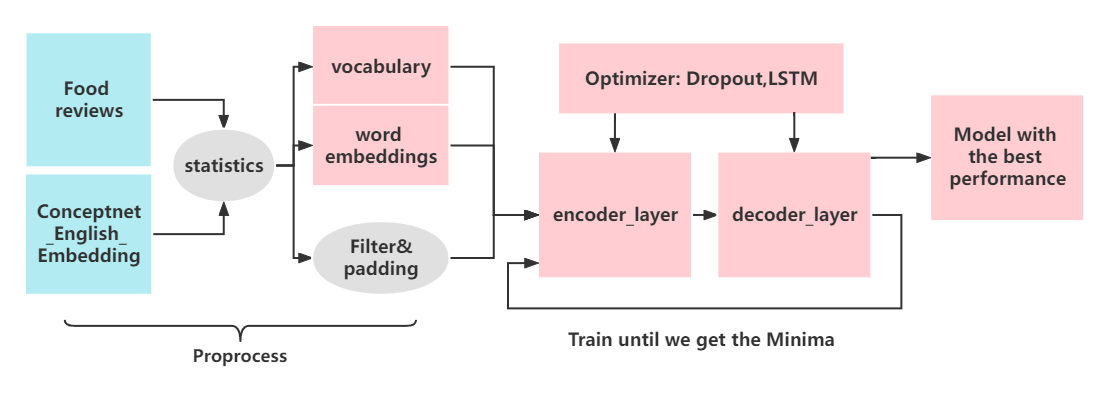
\includegraphics[width=0.5\textwidth]{imgs/System_Structure.png}
\caption{System structure}
\label{fig:System_Structure}
\end{figure}
\subsection{Preprocess}
Our proposed method is to get the basic knowledge from Conceptnet-numberbatch first. Then we check the words in the datasets to generate a vocabulary and get the corresponding embedding by searching the numberbatch. In this way, we get to just initialize very few uncommon words and make the most use of prior knowledge. On the other hand, due to the dependence of RNN on sentence length. We filter some texts that are obviously too long or too short to improve the efficiency of subsequent training. 
\subsection{Model}
Text summarization task is a typical "many to many" task. It's hard to get a precise summary before you scan the entire review. Meanwhile, the reasonable output is usually of indeterminate length. Based on the characteristics of the text summarization task, we design a reasonable RNN structure that contains an encoding and decoding layer. For the encoding layer, we use Bidirectional Recurrent Neural Network(BRNN) to scan the entire reviews from 2 directions, which enables the model to get more comprehensive information. With the LSTM components, full-text information is better concatenated. Those methods make the encoding layer produce more precise knowledge for the downstream tasks. In order to output summary with reasonable length, we apply the dynamic decoder with Seq2seq to ensure the model can automatically adapt to different amounts of text content.

\section{Evaluation Plan}
\subsection{Real datasets}
The dataset we use is Amazon Fine Food Reviews which contains more than 500000 records, spanning a period of more than 10 years. This dataset also provides summaries labeled by humans so that we can train our model to learn this ability to generalize. 
\subsection{Evaluation Measurement}
we will use both metric-based and human-subject evaluations to evaluate our model. Since we get the original summaries in the datasets, we can subjectively judge whether machine-generated generalization results outperform humans.  Besides, the performance of various text summarization methods is reported on shared DUC datasets using an automatic evaluation framework, ROUGE, which is DUC’s official evaluation metric for text summarization. We can also mix DUC with the original dataset and retrain our model to evaluate based on score.
\bibliographystyle{IEEEtran}
\bibliography{references.bib}


\end{document}
